Vision is the ability to make inferences about the natural world from the
patterns of light captured by the eyes of living organism or cameras in
machines. Consider a digital image which is a discrete two dimensional array of
intensity values referred to as pixels. Though each pixel corresponds to a
potentially independent light intensity measurement, in practice pixel
intesities are strongly spatially correlated in natural images. However, this
structure is not caputred by the camera sensor itself; each pixel is stored as
a separate light intensity measurement in memory. Therefore it is natural to 
think of raw images as points in high dimensional space, where the dimension is 
equal to the number of pixels in the image.         

\begin{figure}[ht]
\centering
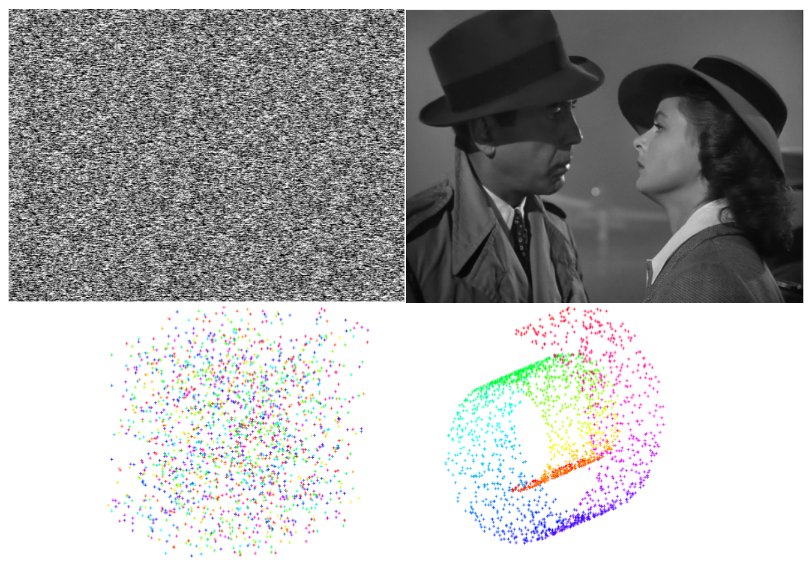
\includegraphics[scale=0.3]{./figures/introduction/structure.png}
\caption{Top left: random image, Top right: natural image, Bottom left:
visualization of unstructured data, Bottom right: visualization of data with
intrinsic structure} \label{fig:LISTA} 
\end{figure}  


It is been a long standing belief in neuroscience that the visual
cortex has a hierarchical organization \cite{hubel1968,felleman1991}. Simply
put, there is a sequence of processing steps which eventually results in our
visual perception of the world. Many recent successes in computer vision have
been attributed to Convolutional Networks, which make use of deep hierarchical
representations heavily inspired by the visual systems of living organism.    
Though these networks are not completely understood, it is clear that 
the sequence of operations corresponding to each layer transforms the data in 
a way that makes the task easier to solve for the final layer, which is often 
a linear operator.    







 
